\documentclass[10pt]{article}
\usepackage[T1]{fontenc}
\usepackage{amsmath}
\usepackage{tikz}
\usetikzlibrary{arrows.meta}
\pagestyle{empty}
% Compile with pdflatex. The page is cropped to the vector artwork.
\newsavebox{\mapbox}
\begin{document}
\begin{lrbox}{\mapbox}
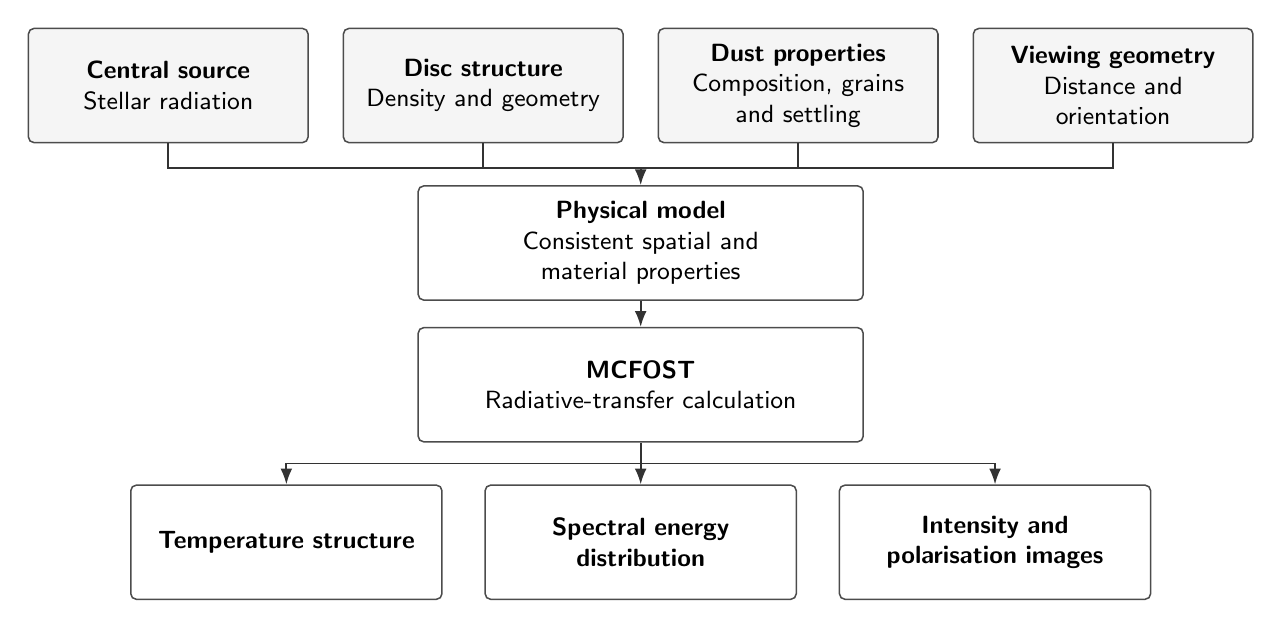
\begin{tikzpicture}[
  box/.style={draw=black!70,line width=0.55pt,rounded corners=2pt,
    align=center,font=\sffamily\small,inner sep=5pt,minimum height=1.45cm},
  inputbox/.style={box,fill=black!4},
  searchbox/.style={box,fill=blue!7},
  arrow/.style={-{Latex[length=2mm]},line width=0.65pt,draw=black!80},
  wire/.style={line width=0.65pt,draw=black!80}
]

\node[inputbox,text width=3.2cm] (star) at (0,0)
  {\textbf{Central source}\\Stellar radiation};
\node[inputbox,text width=3.2cm] (disc) at (4,0)
  {\textbf{Disc structure}\\Density and geometry};
\node[inputbox,text width=3.2cm] (dust) at (8,0)
  {\textbf{Dust properties}\\Composition, grains\\and settling};
\node[inputbox,text width=3.2cm] (view) at (12,0)
  {\textbf{Viewing geometry}\\Distance and orientation};
\node[box,text width=5.3cm] (model) at (6,-2)
  {\textbf{Physical model}\\Consistent spatial and material properties};
\node[box,text width=5.3cm] (rt) at (6,-3.8)
  {\textbf{MCFOST}\\Radiative-transfer calculation};
\node[box,text width=3.6cm] (temp) at (1.5,-5.8)
  {\textbf{Temperature structure}};
\node[box,text width=3.6cm] (sed) at (6,-5.8)
  {\textbf{Spectral energy\\distribution}};
\node[box,text width=3.6cm] (images) at (10.5,-5.8)
  {\textbf{Intensity and\\polarisation images}};
\draw[wire] (star.south) -- (0,-1.05) -- (12,-1.05) -- (view.south);
\draw[wire] (disc.south) -- (4,-1.05);
\draw[wire] (dust.south) -- (8,-1.05);
\draw[arrow] (6,-1.05) -- (model.north);
\draw[arrow] (model) -- (rt);
\draw[wire] (rt.south) -- (6,-4.8);
\draw[arrow] (6,-4.8) -| (temp.north);
\draw[arrow] (6,-4.8) -- (sed.north);
\draw[arrow] (6,-4.8) -| (images.north);

\end{tikzpicture}
\end{lrbox}
\pdfpagewidth=\dimexpr\wd\mapbox+12pt\relax
\pdfpageheight=\dimexpr\ht\mapbox+\dp\mapbox+12pt\relax
\pdfhorigin=0pt
\pdfvorigin=0pt
\shipout\vbox{\offinterlineskip\kern6pt\hbox{\kern6pt\usebox{\mapbox}\kern6pt}\kern6pt}
\end{document}
